\chapter{Propuesta}

Se propone el desarrollo de un sistema que incorpore elementos, tanto de la computación basada en ''trust'' como las de web social, más específicamente, los sistemas recomendadores. El dominio escogido para este sistema es el turismo en la región metropolitana. Actualmente existe una gran variedad de centros culturales y otros lugares interesantes para visitar, sin embargo, un visitante no tiene tiempo para visitarlos todos y además puede tener preferencia sobre algún tipo de lugar por sobre otros. La idea es, primero, ofrecer una plataforma en la que un usuario pueda encontrar lugares culturales cercanos y poder dejar una reseña escrita que describa brevemente la experiencia de la visita. Por otra parte, se espera que las opiniones de la comunidad que use este sistema permitan predecir los lugares que serán del gusto del usuario objetivo. 

\section{Características}
Las principales características que incluye el sistema ''VISIT CHILE'' son 8, entre todas abarcan conceptos de web social, geo-localización y ''trust computing''.

\begin{enumerate}
\item{Posibilidad de dejar opiniones en forma de "reviews" que consisten en una calificación, del 1 al 5 del lugar visitado, junto con una descripción corta del lugar }
\item{Visualización de perfil de usuario, con avatar y lista de "reviews" escritas}
\item{Visualización de lugares culturales, que incluyen una fotografía del lugar, una descripción y además, la lista de opiniones de los usuarios al respecto}
\item{Visualización de lista de lugares recomendados para un usuario, ordenados según el puntaje predicho}
\item{Funcionalidad que permite calificar las reseñas que deja cada usuario, indicando si le fueron útiles o no}
\item{Funcionalidad de tags para cada lugar cultural, según las actividades que se pueden realizar ahí}
\item{Funcionalidad de buscar lugares según el tag que posean}
\item{Funcionalidad de buscar lugares según la cercanía geográfica}
\end{enumerate}

\section{Arquitectura de la solución} 

El sistema ''CHILEEE'' consiste en una aplicación web desarrollada utilizando el framework Ruby on Rails, el cual utiliza el paradigma MVC (Modelo, Vista, Controlador). Para almacenar todos los datos (usuarios, lugares, reseñas y trust) Se utilizó Neo4j, una base de datos NoSQL diseñada para almacenar grafos. Neo4j permite unificar la lógica de trust y la del sistema de recomendación, diseñando el sistema completo como un grafo. En este grafo existen tres tipos de nodos.

\begin{enumerate}
\item{Los de color azul representan a los usuarios, quienes son los que dejarán sus opiniones respecto a los lugares que visitan.}
\item{Los de color verde son los ''Items'', en específico, los lugares culturales sobre los cuales se opina}
\item{Finalmente, los de color rojo son los tags, que describen los lugares, según los tipos de actividades que se pueden hacer en cada uno de ellos.}
\end{enumerate} 
Todo grafo debe tener, además de nodos, arcos, en este caso, representan las relaciones entre las entidades que describe el sistema. Existen cuatro tipos, trust, vote, tagged y review.
\begin{enumerate}
\item{La relación review va desde un usuario hacia un ítem, indica la opinion que tuvo el usuario en particular acerca del item al que apunta. Además de la dirección hacia la que apunta, contiene la información sobre la opinion dada, una corta reseña y una puntuacion en estrellas}
\item{La relación vote describe la opinión de un usario sobre la reseña que haya escrito otro. Ya que una persona no siempre puede estar de acuerdo con la apreciación de otra, se refleja esto en el contenido del arco, que indica si la reseña le fue útil al usuario actual o no.}
\item{La relación tagged es entre un item y varios tags, cuando un tag apunta a un ítem, significa que éste item ha sido ''tagueado'' o ''marcado'' por este tag y es por lo tanto descrito, en parte, por éste. }
\item{La relación trust es entre un usuario y otro, indica el nivel de confianza que uno hacia el otro, el contenido de este arco es un valor que intenta representar el nivel de confianza, un nivel cero significa que no existe confianza, mientras que un nivel 1 indica confianza total. Por defecto el valor asignado es 0.5}
\end{enumerate}

\section{Implementación de las características}

En la sección X se hizo un listado de las características que posee el sistema. A continuación se detallará el diseño e implementación de las características anteriormente nombradas.

\subsection{Estimación de trust} 

Una de las características que hace posible todo es la de escribir reviews. Un usuario registrado puede acceder a cualquier ítem de la base de datos y, si no lo ha hecho ya, escribir una review sobre el lugar que describe el ítem, junto con su puntaje en estrellas, del 1 al 5.

\begin{figure}[hbtp]
\centering
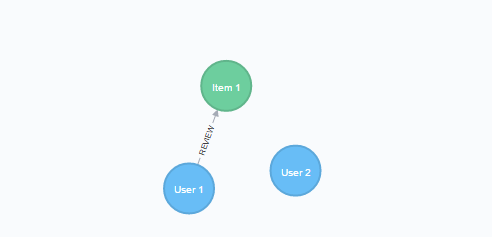
\includegraphics[scale=0.9]{images/grafoej1.png}
\caption{Un ejemplo sencillo de los grafos que genera el sistema. Los nodos azules representan usuarios, mientras que los nodos verdes representan los ítems (lugares culturales) a evaluar. El arco que une al Usuario 1 con el Item 1 es la reseña (Review) que le da el usuario al ítem.}
\end{figure}

Ya que el usario pertenecerá a una amplia comunidad, repartida entre varias comunas de la RM, no es posible garantizar que conozca personalmente a cada otro usuario del sistema. Además, dado que la información disponible sobre otras personas es limitada, ya que la única forma de interacción entre usuario que se permite es la escritura de reviews, se hace apropiado que se estime la confianza según el nivel de acuerdo que exista entre las opiniones de los usarios. Por lo tanto, se implementó un sistema que permite valorar como útil o poco útil la opinión de otro usuario. El usuario puede hacer ésto al hacer clic en la mano con dedo pulgar hacia arriba o la que apunta hacia abajo.

\begin{figure}[hbtp]
\centering
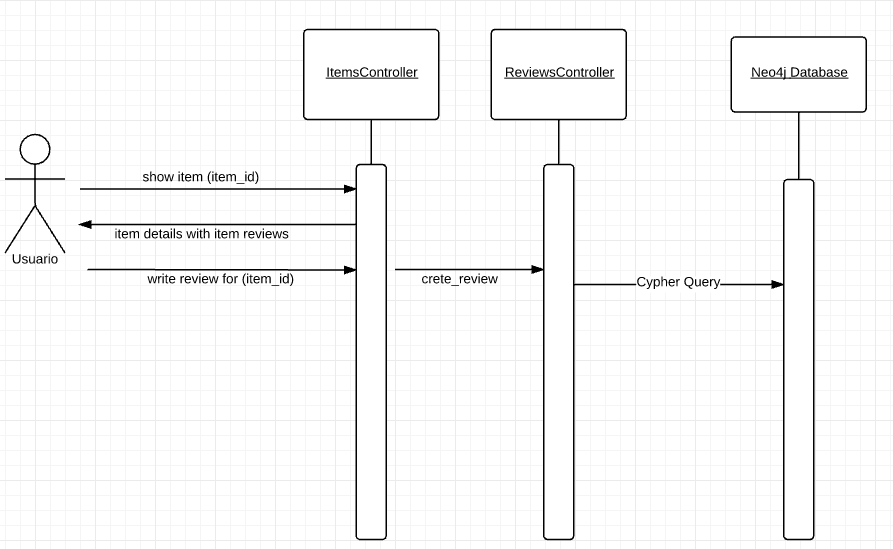
\includegraphics[scale=0.8]{images/review_history.png}
\caption{Diagrama de interacción entre el usuario, los controladores y la base de datos}
\end{figure}

Para ejemplificar, se utilizarán 3 usuarios de ejemplo: Usuarios A y B

Suponer que el Usuario A ingresa a la vista de un item arbitrario, dentro del cual hay sólo una reseña, escrita por el usuario B. Ahora imaginar que el usuario A está de acuerdo con lo que el usuario B escribió y decide valorar positivamente su reseña. A partir de ésto hay dos casos posibles:

\begin{enumerate}
\item{Si el usuario A y el usuario B no tenían relación de trust existente, se crea una entre ambos, con el valor por defecto, 0.5}
\item{Si el usuario A y el usuario B ya tenían una relación de trust, ésta se refuerza y se aumenta el valor de trust de A hacia B en 0.1. Si la valoración hubiese sido negativa, se habría restado 0.1 al trust de A a B.}
\end{enumerate}

De esta manera, se pretende un acercamiento a como funciona la confianza en la vida real, no de forma binaria (confiar o no confiar), sino más bien, de forma gradual. 

\subsection{Estimación de ítem recomendado}

Uno de los pilares fundamentales del sistema es el algoritmo que permite obtener los ítems recomendados. Para ésto, después de evaluar las opciones posibles (ver estado del arte) se decidió por una variante del algoritmo collaborative filtering (encontrar nombre exacto) que incluye el factor de confianza como variable a considerar. En palabras simples, el sistema intenta predecir el puntaje que el usuario objetivo dará a cierto ítem en partícular, los ítems que reciban mayor puntaje serán los recomendados. A continuación se explica en detalle su funcionamiento.


\begin{figure}[hbtp]
\centering
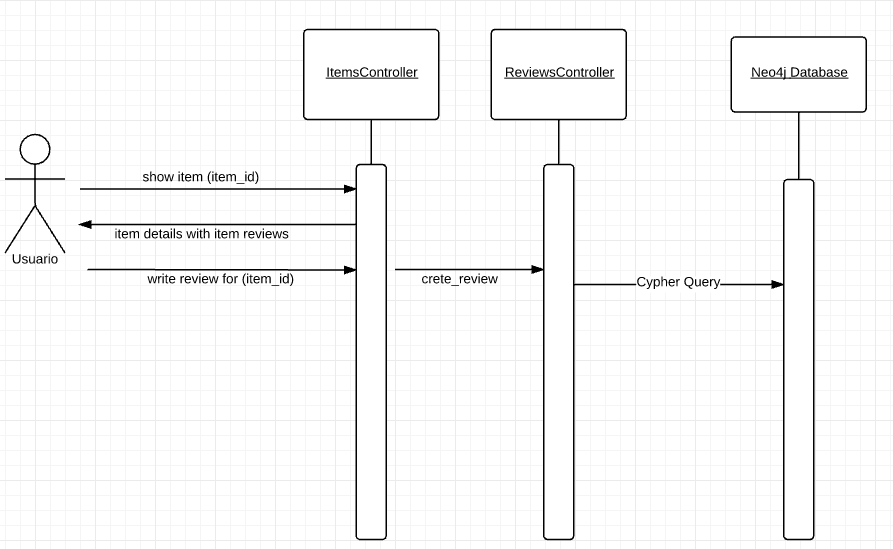
\includegraphics[scale=0.8]{images/review_history.png}
\caption{Diagrama de interacción entre el usuario, los controladores y la base de datos}
\end{figure}

Cuando un usuario ingresa al sistema usando sus credenciales, el controlador de usuarios hace una redirección hacia la función de recomendar. La cual calcula los puntajes predichos para todos los ítems candidatos con la siguiente fórmula 

\begin{equation}
pred(u,i) = \overline{r} + \frac{\sum\limits_{vecindario} Sim(u,n) * (r_ni - \overline{r_n} )}{\sum\limits_{vecindario} Sim(u,n)}
\end{equation}

Donde $Sim(u,n)$ es la similitud entre el usuario $u$ y el usuario $n$, $\overline{r}$ es el rating promedio (de todos los usuarios) , $r_ni$ es el rating que da el usuario $n$ al ítem $i$ y $\overline{r_n}$ es el rating promedio que entregó el usuario $n$. 

Para facilitar la comprensión del funcionamiento del algoritmo, se va a usar el siguiente ejemplo:

\begin{figure}
\centering
\begin{adjustbox}{max width=\textwidth}
\begin{tabular}{l*{6}{c}r}
                  & Plaza de Armas & Cerro Sta. Lucia & Cerro San Cristobal & Museo de Bellas Artes & Quinta Normal  & Teatro Municipal & Centro GAM \\
\hline
Juan          & 5 & 4 & 2 &   & 1 &   &   \\
\hline
Ignacio       & 3 &   & 2 &   & 5 &   & 4 \\
\hline
Perla         & 3 & 3 &   & 1 & 4 & 3 &   \\
\hline
Inés          & 5 & 5 &   & 1 & 2 &   & 5 \\


\end{tabular}
\end{adjustbox}
\caption{Las estrellas que dan los usuarios A, B, C y D a distintas películas}

\end{figure}

En este ejemplo, el usuario que entra al sistema y cuyos puntajes son predichos se conoce como consumidor, en este caso es el Usuario 1.

Cada ítem para el cual el consumidor aún no ha escrito una review y que se encuentre a cierta distancia geográfica es un potencial ítem recomendado, pero antes es necesario conocer qué puntaje le asignaría el consumidor.

\begin{figure}
\centering
\begin{adjustbox}{max width=\textwidth}
\begin{tabular}{l*{6}{c}r}
                  & Plaza de Armas & Cerro Sta. Lucia & Cerro San Cristobal & Museo de Bellas Artes & Quinta Normal  & Teatro Municipal & Centro GAM \\
\hline
\rowcolor{yellow} Juan          & 5 & 4 & 2 &   & 1 &   &   \\
\hline
Ignacio       & 3 &   & 2 &   & 5 &   & 4 \\
\hline
\rowcolor{yellow}Perla         & 3 & 3 &   & 1 & 4 & 3 &   \\
\hline
\rowcolor{yellow}Inés          & 5 & 5 &   & 1 & 2 &   & 5 \\


\end{tabular}
\end{adjustbox}
\caption{La misma tabla de la figura x, imaginar que se quiere conocer el puntaje que Juan dará al Museo de Bellas Artes, para eso se deben tener en cuenta sólo los usuarios que hayan visitado este lugar, o sea, Perla y Inés.}

\end{figure}

El proceso de calcular el puntaje predicho para cada ítem se conoce como sesión. Como se puede notar, cada ítem candidato implica una sesión de recomendación.

Comenzando por el primer ítem candidato, al iniciar la sesión, el sistema consulta por todas las reviews que hayan sido escritas sobre el ítem actual. Los usuarios que escribieron estas reviews se conocen como productores.

De este grupo de productores, se escogen sólo los que hayan escrito reseñas sobre al menos dos ítems sobre los que el consumidor haya también dado su opinión.
\newcolumntype{g}{>{\columncolor{yellow}}c}
\begin{figure}
\centering
\begin{adjustbox}{max width=\textwidth}
\begin{tabular}{|c|g|g|c|c|g|c|c|}

                  & Plaza de Armas & Cerro Sta. Lucia & Cerro San Cristobal & Museo de Bellas Artes & Quinta Normal  & Teatro Municipal & Centro GAM \\
\hline

Juan          & 5 & 4 & 2 &   & 1 &   &   \\

\rowcolor{white}Ignacio       & 3 &   & 2 &   & 5 &   & 4 \\

Perla         & 3 & 3 &   & 1 & 4 & 3 &   \\

Inés          & 5 & 5 &   & 1 & 2 &   & 5 \\


\end{tabular}
\end{adjustbox}
\caption{Tabla x, pero destacando que para el cálculo del puntaje al Museo de Bellas artes, sólo se tomaran en cuenta lugares que hayan sido visitados por los tres usuarios, Juan, Perla e Inés.}

\end{figure}


En la sección de estado del arte se describieron varias formas en que se pueden integrar los algoritmos de recomendación con los de trust. Para este dominio en particular, ya que se intenta hacer un acercamiento al comportamiento observado en la vida diaria entre personas, se decidió que se utilizará el trust como un umbral, en el que la opinión de una persona ''no confiable'' se considera inválida y por lo tanto, es ignorada. 

Por lo tanto, después de determinar los posibles usuarios productores, existe otro filtro que determina quiénes serán de confianza. Después de obtener la lista inicial de productores, se determina el nivel de trust que tiene el consumidor con cada uno de los productores. Si no existe una relación directa de trust entre el consumidor y el posible productor, ésta se calcula mediante ''tidal trust''. Una vez que se tiene el valor de trust, el productor candidato es removido de la lista si es que su trust con el consumidor es menor a 0.5, en caso contrario, permanece en la lista. 

Luego, para estimar numéricamente el parecido de las opiniones del consumidor con cada productor, se utiliza la correlación de Pearsson (cita). La idea detrás de esta lógica es que mientras más parecido sea el consumidor con un productor, más peso tendrá éste sobre la estimación del puntaje predicho. Empezando por Juan y Perla:

\begin{figure}

\begin{equation}
sim(u,n)=\frac{\sum_{i=1}^{n}(u_i-\bar{u})(n_i-\bar{n})}{\sqrt{\sum_{i=1}^{n}(u_i-\bar{u})^2}+\sqrt{\sum_{i=1}^{n}(n_i-\bar{n})^2}}
\end{equation}
\caption{La similitud entre dos conjuntos, según la correlación de Pearsson, en este caso, interpretar los valores de $u$ como las estrellas que ha dado Juan a los lugares que visitó y los de $n$ los que ha dado Perla. }

\end{figure}
Conociendo el puntaje que ha puesto en promedio cada productor, $\bar{u}$ para Juan y $\bar{n}$ para Perla, se calcula la diferencia con el puntaje dado. Reemplazando con los promedios y los valores de reseñas, se tiene:





Este proceso se repite para cada dupla de consumidor-productor posible.

Con esto, se tiene el numerador de la ecuación (referencia), el denominador es más sencillo de calcular, ya que sólo es la diferencia entre afsd.

Con esto, se llega finalmente a un puntaje estimado, que dará el consumidor al ítem actual. Este proceso se repite para cada ítem candidato.
Luego, cuando ya se tienen todos los puntajes predichos, se considera como recomendables sólo los ítems cuyo puntaje estimado sea al menos 3 estrellas.

%diagrama ejemplo, con alguno descartado.

Son estos los ítems que el sistema va a mostrar en la vista de recomendados, ordenados de mayor a menor puntaje. 






